\documentclass[a4paper,twoside]{article}


\usepackage{epsfig}
\usepackage{subcaption}
\usepackage{calc}
\usepackage{amssymb}
\usepackage{amstext}
\usepackage{amsmath}
\usepackage{amsthm}
\usepackage{multicol}
\usepackage{pslatex}
%\usepackage{natbib}
%\let\bibhang\relax
\usepackage{apalike}
\usepackage[bottom]{footmisc}
\usepackage{SCITEPRESS} 


\usepackage{hyperref}
\usepackage{graphicx}
\usepackage{listings}
\usepackage{float}
\usepackage[T1]{fontenc}
\usepackage{inconsolata} % For cleaner fonts in code listings
\usepackage{bm}
\usepackage{bold-extra}
\usepackage{adjustbox}

\hypersetup{
  pdftitle = {Needles in a Haystack: Using PORT
  To Catch Bad Behaviors Within Application Recordings },
  pdfkeywords = {Domain Specific Languages,
                 Programming Languages,
                 Event Processing,
                 Automated Testing,
                 Stream Processing,
                 Software Reliability,
                 Software Testing},
  pdfauthor = { Names removed for anonymous submission},
  bookmarksnumbered,
  bookmarksopen=true,
  colorlinks=true,
  urlcolor=[rgb]{.35,0,0},
  linkcolor=[rgb]{.35,0,0},
  citecolor=[rgb]{.35,0,0},
  pdfstartview={FitH},
}


\input{annotations}

% Format code
\lstdefinelanguage{PORT}{
  keywords={event,type,with,and,not},
  morecomment=[l][\color{green!60!black}]{\#}
}
\lstset{
language=PORT,
breaklines=true,
backgroundcolor=\color{white},
numbers=left,
xleftmargin=1.1em,
numbersep=5pt,
%escapeinside={@}{@},
numberstyle=\tiny\color{gray},
basicstyle=\small\ttfamily,
columns=fullflexible,
mathescape=true,
showspaces=false,
}


\begin{document}


\title{Needles in a Haystack: Using PORT to Catch Bad Behaviors within
Application Recordings}

\author{\authorname{Preston Moore\sup{1},
Thomas Wies\sup{1},
Marc Waldman\sup{2},
Phyllis Frankl\sup{1}, and
Justin Cappos\sup{1}}
\affiliation{\sup{1}New York University, \sup{2}Manhattan College}
}

%}
\keywords{Domain Specific Languages, Event Processing, Environmental Bugs}

\begin{abstract}

Earlier work has demonstrated that,
when evaluating the quality of a piece of software,
there is tremendous value in
information that can be extracted
from recordings
of an application's activity.
The trick is in how to extract it.
Applications often make hundreds or thousands of requests
to external entities over the course of an execution
which makes it difficult
to recognize and respond to important patterns.
Existing event processing applications,
used successfully in fire alarms,
industrial control systems,
and computer network monitoring software,
have emerged as a potential solution
to this problem.
By design,
these systems
search
incoming streams of events
for a sequence,
and
react appropriately
when a pattern occurs.
Thus,
if application actions
can be processed like events,
this technology could be harnessed
as a tool for identifying bugs.
In this work,
we demonstrate
how
the creation of
a new domain specific language
called CSlang
allows users
to not only construct a program that describes an activity,
but also to rewrite an input activity stream on the fly.
The former may be used
to identify application activity
that may indicate the presence of a bug,
while the latter produces a modified stream
that may be used
for more active testing.
Using CSlang makes it easy
to identify sequences
in streams like event logs,
remote procedure call traces,
or system call activity.
To see how our efforts compared against other work
We employed CSlang
in recreating the mutators and checkers
used by
the SEA technique,
a project introduced in 2019
that was able to find bugs
by modifying and replaying the results of
an application's system calls.
We found our re-implementations
achieved the same efficacy
and better reliability
while consisting of XX\% less lines of code.
We further illustrated CSlang's extensibility
by adding support for remote procedure call traces
and creating programs that
could examine and rewrite the contents of
these recordings.

\end{abstract}

\onecolumn \maketitle 
\normalsize \setcounter{footnote}{0} \vfill


\section{Introduction}
\label{SEC:introduction}

\textit{Clever quote here}


Environment also contains separate components of the same application
that must communicate with one another

With the explosion of...

...applications are no longer single units sitting on a specific machine.

In fake study 1, researchers estimate that XX\% of distributed applications
contain bugs...

...recent very bad environmental bug~\cite{devzeroroot}


%No matter how well an application is tested before its release,
%new bugs always seem to emerge after deployment.
%In fact, Oracle estimates that 40\% of deployed applications
%contain critical defects -- a fact that is compounded that deployment
%increases the cost to fix these flaws by 100 times~\cite{OracleAppQuality}.
%One reason for this behavior
%is that these applications will operate within a diverse set of
%deployment \emph{environments},
%and variations between these environments tend to
%reveal previously undiscovered flaws.
%These flaws emerge from
%such factors as
%operating system APIs changing across versions
%~\cite{LinuxGlibcChanges},
%or small variations in file systems exhibiting subtle but critical
%differences~\cite{EXT4Layout, AppleHFS}.
%Even if the network and adapter are identical,
%network behavior can still diverge from what is expected~\cite{vbox},
%and these environmental differences greatly exacerbate
%the chance that an application will function incorrectly when deployed.

...something something something applications made of multiple
intercommunicating modules.


...This is increasingly true today's applications that typically consist of
multiple, intercommunicating modules


...These complex bugs are often difficult to reason about...


%These unforeseeable bugs
%complicate the work of application developers who, according to a
%recent survey conducted by ClusterHQ~\cite{ClusterHQSurvey},
%spend a significant portion of their time
%debugging errors that only appear in production.
%Numerous efforts have been made to reduce this burden.
%One approach
%is to hide environmental differences behind standard interfaces.
%Unfortunately,
%even specialized ``Write-Once, Run Anywhere'' environments
%that attempt to hide these differences,
%such as the Java Runtime Environment,
%are not perfect,
%leading them to be rechristened ``Write-Once, Debug Everywhere''~\cite{WODE}.
%A more direct approach would be
%to identify and fix deficiencies before deployment,
%but history has shown that,
%even if enormous effort is put forward,
%it may be insufficient to uncover these bugs.
%Microsoft employs thousands of engineers with nearly a
%1:1 ratio of testers to developers~\cite{Page2009}.
%Yet, a recent Windows Update released
%in response to the Spectre Intel CPU vulnerability
%resulted in machines with certain hardware configurations
%being rendered unbootable~\cite{kb4056892}.


%twe introduced Simulating Environmental Anomalies (SEA)
%and its key insight that
%problematic environmental properties,
%which we refer to as \textit{anomalies},
%can often be detected
%in the function calls,
%system calls,
%or other communications an application makes within an environment.
%When employing SEA,
%the anomalies
%unique to a given environment
%can be inserted into
%the communications of an application under test
%in such a way
%that its responses will indicate potential
%for failures upon deployment.
%These anomalies can be preserved and cataloged
%allowing them to be reused to test other applications,
%without requiring
%per-application effort.
%Over time,
%a corpus of environmental anomalies can be assembled
%that can help ensure
%future applications do not suffer from bugs of the past.


In earlier work, we made an initial thrust at this problem by employing the
Simulating Environmental Anomalies (SEA) technique on the system calls an
application makes. Our effort centered on the key insight, that problematic
environmental properties, known as anomalies, are visible in the
communications between the components that make up an application.  The
work documented in this paper augments SEA so that its proven methodology
can be used to test a broader set of applications.  Our improvements take
SEA beyond system calls by providing by providing a more generic way to
encode and simulate anomalies across the set of applications that use
structured communications like remote procedure calls.
This allows anomalies that were
valuable in testing one application to be directly used to test other
applications with similar communication strategies.  In effect, this takes
SEA's capability at finding environmental bugs and applies it to other bug
domains while both maintaining existing advantages of SEA and
dramatically improving its reach.




In order to evaluate our improvements to SEA, we needed a way to express
anomalies that was not tied to a particular domain.  To this end, we
implemented a new programming language, CSLang.  CSLang is a simple, but
powerful, language for describing the transducers needed to both identify
simulation opportunities and carry out the transformations required to make
said simulations a reality.  Initially, we used CSLang to implement the
mutators previously described in \preston{however you cite the first paper
here}. We found these mutators outperformed in terms of SOME METRIC HERE and
in XXX\% fewer lines of code.  To further our evaluation, we implemented ZZZ new
mutators capable of simulating anomalies in applications that use either
JSON-RPC or XML-RPC.  We employed these mutators in testing suitable
applications that ranked highly on Debian's popularity contest.  This
exercise identified AAA new bugs in the tested applications.  In the
future, these mutators can be used on similar application to expose more
bugs without additional test writing effort.

%In addition to demonstrating that
%CrashSimulator could find bugs, we were also able to
%show that developers with varying backgrounds
%could use the tool
%on real world applications with ease.
%We conducted a user study with
%12 undergraduate and graduate computer science students
%who were asked to use CrashSimulator to test
%the same type of applications evaluated in our initial tests.
%The results show that the developers were able to find bugs
%that were missed by the applications' existing testing strategies.
%Additionally, the
%participants were able to find bugs
%in environments with which they had only a limited amount of experience.

The main contributions in this work can be summarized as follows:

\begin{itemize}

\item{An expanded version of the Simulating Environmental Anomalies (SEA)
  technique that can expose bugs both between an application and its
    environment and between application components that communicate with
    one another}

\item{It demonstrates a new language, {\em CSLang},
which allows for concise descriptions of transducers that may
modify streams of communication between components in order to simulate
anomalous conditions}

\item{It proves the value of CSLang by illustrating the ease with which
  transducers can be constructed and the effectiveness with which they are
    able to find bugs in real world applications }

\end{itemize}

\section{Background and Motivation}
\label{SEC:background}

\subsection{The Problem of Environmental Bugs}

\textit{But it works on my machine!} goes the refrain of the tortured
software developer whose application works correctly when executed on a
development computer only to fail once it is deployed.  This occurs with
such frequency that the ``works on my machine'' phenomenon is a well known
source of pain
and frequent topic of discussion
in software and project management
literature~\cite{notreal}.
The problem is so widespread
that FAKESTUDY concluded
that \$XXX are spent annually on efforts to
recall,
fix,
and re-deploy applications
because of all the bugs
that slipped past extensive testing efforts
during development.

Earlier work has demonstrated that environmental bugs, those that occur due
to unanticipated qualities external to an application, are a major source
of such failures.  This fact continues to be reinforced by the regular
appearance of high impact environmental bugs in major pieces of
software~\cite{devzeroroot}.  And it appears that no class of application
is safe with environmental bugs affecting operating systems~\cite{bad},
user applications~\cite{bad} and even web applications~\cite{bad} in the
last year alone!

\subsection{Our Motivating Example}

An initial thrust was made at this problem by Moore et al
when they employed
the Simulating Environmental Anomalies (SEA) technique
on applications' system calls~\cite{crashsim}.
This effort centered on the key insight
that problematic
environmental properties,
known as anomalies, are visible in the
communications between the components that make up an application.
They found that,
once captured,
these anomalies
could be
used to create simulations
that test
an application as if
it had encountered the captured anomalies
in the real world.
But system calls are just part of the story.
This paper documents an effort to augment SEA
so that its proven methodology
can be used to test a broader set of applications.
Our improvements
apply SEA's existing capability
to new bug domains
while maintaining its existing advantages and
dramatically
improving its reach.


\subsection{Why a New Programming Language?}
\begin{figure}
  \includegraphics[scale=.50, frame]{images/cslanglisting}
  \caption{A listing of a cslang program.  This program finds situations
  where a program opens a file and closes it without reading from it.  In
  such instances, it modifies the return value close call to be -1,
  indicating failure.}
  \label{fig:cslanglisting}
\end{figure}

\begin{figure}
  \includegraphics[scale=.50, frame]{images/flinklisting}
  \caption{A listing of an Apache Flink program that does the same thing as the
  cslang program... I need to figure out what comparison stuff to put in
  this caption.}
  \label{fig:flinklisting}
\end{figure}


The decision to create a new programming language was not one we
undertook lightly,
as such an effort takes
a significant amount of work
to define,
implement, document, and support.
In this section we discuss the features we needed for this work
and why existing systems fell short.

First, we needed a language that treated state as a first-class citizen.
That is, it must allow the internal contents of events like argument data,
pointer addresses, and return values to be easily captured, manipulated, and
reused in subsequent operations.
This is necessary because,
at a very high level,
the purpose of system calls,
function calls,
rpc calls,
or other similar activity
is to allow an application
to gather data from an external module like a library or the operating
system.
As a result, it is frequently useful to be able to store the data returned by
one such action, modify it, and use it in matching actions.
For example, one may store the file descriptor returned by a {\tt
socket()} system call and use it later to match other related
communication system calls.
We found that this sort of usage was common across many types of
application activity further reinforcing our desire for a language that was
closely tailored to our needs on this in this area.

% Need to support new event stream formats easily?


\preston{We need to make sure we have given a best effort at shortening and
optimizing code from other languages with which we are making comparisons}

Our second requirement appears to be largely aesthetic at first glance
but there is a
larger purpose -- ease of learning and ease of use.  CSlang offers
improvements over existing languages along two primary fronts.
First, many event processing languages are verbose.
Consider figure~\ref{fig:cslanglisting}  which shows a
CSLang program that matches sequences where an application opens and closes
a file without reading from it.  When such a sequence is found, it is
modified such that the {\tt close()} call returns -1, indicating failure.
The main work of this program is performed in just four lines of CSlang
code.  For comparison, figure~\ref{fig:flinklisting} contains a Java program that
implements an approximation of the same program that was implemented in
CSlang~\ref{fig:cslanglisting}.
This program is only an approximation because it does not modify the return
value of the close() call as the CSLang program does.  Further, it assumes
that other work has been done to modify Apache Flink to enable the
consumption of a sequence of system calls.
In spite of these shortcomings, comparing the two programs remains
enlightening.  The Flink program is harder to read because it contains a
great deal of boilerplate code
that cannot be avoided due to its dependence on a fully-featured
programming language.  Other work that explores how developers read and
understand (or mis-understand!) code has shown that such constructs obscure
a programs meaning, harming understanding and
maintainability~\ref{CITEATOMSWORK}.
In light of this, we believe the benefits of a
new programming language
focused on allowing its users to get a lot of work done
with a small amount of easily-readable code are evident.

The second front involves CSlang's programming paradigm.
While other event processing languages tend toward functional or
declarative programming,
CSlang programs more closely follow an imperative programming style.
We came to this decision because studies
have shown that developers are more likely to be familiar and comfortable
with such a paradigm~\cite{XXXX}.  We believe this will make it easier for
developers to learn the language, foster greater popularity, and it aligns
with the goals presented in our motivating example.

Our final requirement is, perhaps, the most important.
We want CSlang programs to be capable of more than simply matching
a pattern of events and indicating that it has occurred.
Our review of the work on the SEA technique has shown that the ability to
{\textit modify} is central to forcing an application into situations where
it may fail rather than only passively monitoring for it to perform
problematic sequences.  While the feature-rich nature of several related
languages and libraries means it is likely possible to modify and output
incoming events, it is by no means a straightforward
and ergonomic experience.
Constructing CSlang to support output as a primary feature allows us to
easily describe the types of transformations needed to expose bugs.



\vspace{-.75cm}
\section{Language Overview}
\label{sec:Overview}

\begin{figure}[h]
  \centering
  \includegraphics[scale=.6]{images/processing}
  \caption{A mutator individually processes each item in an input
  sequence, updating it's internal state and producing output according
  to the rules described in its program.}
  \label{fig:Processing}
\end{figure}

The purpose
of a CSlang program is to completely describe a mutator
that both
accepts a chosen stream if it contains a particular
activity sequence and can produce a modified
output stream
for application testing.
Because a mutator is essentially a
transducer enhanced to operate over complex data structures
rather than symbols in a string
this description must cover all states,
the associated output of those states,
and the transition
relation that ties them all together.
Simply enumerating every aspect of a mutator could be very verbose
so we intentionally tailored CSlang's semantics to allow its users to
describe complex configurations in a concise manner.
In this Section we cover the design decisions we made
to achieve this goal.
Section~\ref{sub:ProcessingEventStreams} describes how executing a program works
while
in Sections~\ref{sub:PreambleAndBody}~and~\ref{sub:SyntaxAndSemantics},
we discuss the
language's syntax and semantics and illustrate the details
of these properties
with small examples.
Section~\ref{sub:DatawordOperators} takes a more
detailed look at important operators.

\subsection{Processing and Event Streams}
\label{sub:ProcessingEventStreams}
CSlang was written to
apply event processing
techniques to application activity
in order to catch bugs and drive further
testing.
To accomplish this, a CSlang program maps this activity onto an
event stream
made up of a chronological listing of the function calls, library
calls, system calls, or other structured requests made by the program.
Within this stream each element consists of two pieces: a unique
identifier and a set of parameters.
This arrangement allows a user to find
a specific category of events
in a stream
by matching a set of desired properties.
The system makes the match by specifying
an identifier and a set of parameter value
constraints.  For example, an unsuccessful {\tt close()} call could be
found by looking for events with the identifier {\tt close} and a return
value of -1.  This pairing of an identifier and a set of parameter
constraints, known as a dataword, forms the primary mechanism in CSlang for
selecting specific events out of an activity stream.

Building on this, we can use datawords to implement the method by which
a CSlang program is able to
identify a  pattern of activity.
The general process, illustrated in Figure~\ref{fig:Processing}, goes like
this.  A pattern is encoded as a list of datawords, and compared against
events from the
input event stream until the first dataword
finds a ``match'' (matching is discussed further in
Section~\ref{sub:PreambleAndBody}).  The event stream is next matched
against the
second dataword
and so on until all datawords have been matched or the event stream is
exhausted.


%% talk about output.
%Output is achieved through one further addition -- an output clause.  This
%clause may be applied to any of the datawords in the list and describes
%what output should be produced when the dataword it is associated with
%matches an event.
%
%Datawords without an output clause are simply output without modification.
%
%In the following sections we discuss how these elements may be written as a
%CSlang program and transformed into a working mutator.


\subsection{Preamble and Body}
\label{sub:PreambleAndBody}

\begin{figure}[h]
\centering
\begin{tabular}{c}
\begin{lstlisting}
########## Preamble ##########
event statbuf {dev: String@0, stino: String@1, mode: String@2};
event fstat {fd: Numeric@0, st: statbuf@1};
##############################

##########   Body   ##########
finddev <- "st_dev=makedev(0, 4)";
findino <- "st_ino=4026532069";
out1 <- "foo";
out2 <- "bar";
fstat({st: {dev: ?finddev, stino: ?findino}});
fstat({st: {dev: !finddev2, stino: !findino2}});
fstat({st: {dev: ->out2, stino: ->out2}});
##############################
\end{lstlisting}
\end{tabular}
\caption{An example CSlang program with its preamble and body sections
  labeled.}
\label{lst:PreambleBody}
\end{figure}



A CSlang program can be divided into two sections: the preamble and the body.
Figure~\ref{lst:PreambleBody} shows an example program with these sections
labeled.
The preamble defines the sorts of events
expected
to appear in an input event stream and the set of parameters
under which future datawords will operate.  Specifying this information
up-front configures a CSlang mutator to
automatically ignore extraneous information from the incoming stream.  This
means that subsequent body statements only have to deal with events and
parameters pertinent to the goal of the program.

The body of a CSlang program consists of a list of datawords that
are responsible for configuring the states and transitions
that will be included in the mutator a CSlang program describes.
Each dataword (excluding usages of the NOT operator, discussed further
in~\ref{subsub:NOT}) configures a single
state and the rules that govern transitioning into it.
In order for a mutator to transition into a new state
the current event must ``match'' the requirements of the destination state.
In CSlang, a match requires satisfying three rules:

\begin{itemize}
\item{The event's identifier must match the destination state's identifier}
\item{All parameters with the match operator applied must have a value equal to
  the value currently stored in the associated register (discussed further
    in Section~\ref{sub:DatawordOperators})}
\item{All predicates must be satisfied by the parameter values in the
  current event}
\end{itemize}




\subsection{Syntax and Semantics}
\label{sub:SyntaxAndSemantics}

Figure~\ref{lst:SyntaxGrammar} contains a simplified
version of CSlang's grammar.

\begin{figure}[h]
\centering
\begin{tabular}{c}
\begin{lstlisting}
S: statementlist
statementlist: statement*
statement: eventdefinition
           | variantdefinition
           | assignment
           | dataword
eventdefinition: id (id_1, t_1, l_1), ..., (id_n, t_n, l_n)
variantdefinition: var_id ed_1, ..., ed_n
assignment: x <- e
dataword: id paramexp predexp outputexp
paramexp: (pid_1, op_1, regid_1), ..., (pid_n, op_n, regid_n)
predexp: (lhs_1, cmp_1, rhs_1), ..., (lhs_n, cmp_n, rhs_n)
outputexp: id paramexp
e \in Expr := e_1 + e_2 | e_1 - e_2 | ...
\end{lstlisting}
\end{tabular}
\caption{This is a listing of CSlang's grammar with some implementation
  details omitted in order to improve readability.}
\label{lst:SyntaxGrammar}
\end{figure}


\begin{quote}
\centering
\textbf{S: statementlist}
\end{quote}

This production triggers the creation of a mutator with only a starting
state.  This state is accepting in two situations:
\begin{itemize}
  \item{When no other states are added to the automaton by subsequent
    statements}
  \item{When the only other states added to the automaton are NOT states
    which reject sequences they match}
\end{itemize}
In all other cases this is a rejecting state that produces no output.

\begin{quote}
\centering
\textbf{assignment: x <- e}
\end{quote}

Assignment statements store the value of an expression, e, into a named
register on the mutator being described.
If the register does not exist,
it is created;
otherwise its stored value is overwritten.
Registers may contain Numeric or String values.  Register contents
may be used in subsequent statements to specify parameter values that must
be present in order for an event to match or as values to be output.

\begin{quote}
\centering
\textbf{eventdefinition: id (id\_1, t\_1, l\_1), ..., (id\_n, t\_n, l\_n) }
\end{quote}

\begin{figure}[H]
\centering
\begin{tabular}{c}
\begin{lstlisting}
event statbuf {dev: String@0, stino: String@1, mode: String@2};
event fstat {filedesc: Numeric@0, statstruct: statbuf@1};
\end{lstlisting}
\end{tabular}
\end{figure}

An event definition statement describes an event that could appear in an input
stream.  Each statement specifies an event ``variety'' and a list of
parameters that should be accessible in later dataword statements.
An event's variety will correspond
with the system call name, RPC call name, or, in the case of other activity
representations, a unique identifier that allows events of the same
variety to be picked out of a stream.

The second line in the above example shows an event
definition for
the {\tt fstat()} system call
with two parameters:
a numeric file descriptor, the system call's first parameter,
and structure named statstruct
which is the system call's second parameter.
The first line in the above defines statstruct's layout.


\begin{quote}
\centering
\textbf{variantdefinition: var\_id ed\_1, ..., ed\_n}
\end{quote}

\begin{figure}[H]
\centering
\begin{tabular}{c}
\begin{lstlisting}
event bothread {read filedesc: Numeric@0} | {recv filedesc: Numeric@0};
\end{lstlisting}
\end{tabular}
\end{figure}

A variant definition allows several event definitions to be combined under
a single identifier.  This identifier may then be used in a dataword
statement to match any of the collected events.  This feature arose as a
result of situations where one of several system calls could be used to
perform the same operation (e.g. {\tt read()} and {\tt recv()}).  The
concrete syntax necessary to achieve this pairing is shown in the example
above where the variant ``bothread'' is defined such that it will match
either a {\tt read()} or {\tt recv()} system call.

\begin{quote}
\centering
\textbf{dataword: id paramexp predexp outputexp}
\end{quote}

\begin{figure}[H]
\centering
\begin{tabular}{c}
\begin{lstlisting}
fstat({statstruct: {dev: !finddev2, stino: !findino2}})
with filedesc == 4 and statstruct.dev == "st_dev=makedev(0, 4)"
-> fstat({filedesc: ->fdout2});
\end{lstlisting}
\end{tabular}
\end{figure}

Dataword statements are responsible for adding new states to the
mutator.  This means they must specify any register operations,
transition conditions, and output associated with these new states.  To
tackle this complexity we will address each part of this production
individually.

\textit{id paramexp}

The parameter expression offers an opportunity to examine and store
parameter values from the current event.  CSlang supports two operators
that may be applied to parameter expression members.  The match operator
(!) allows for the rejection of otherwise matching events
by enforcing a required value on a
chosen parameter while the store operator (?) copies a value from the
current event and stores it in the specified register.


\textit{predexp}

Predicate expressions are used to place additional restrictions that must
be met if the mutator is to advance into the newly created state.  These
restrictions compare values from the current event to either register
values or literal values.

\textit{outputexp}

An output clause controls the output that will be produced when its
associated state is entered.  The nature of this output is controlled by a
parameter expression that specifies which parameters of the current event
should be replaced with a value from a register.  If a parameter is not
included in the parameter expression, its original value is used.
Similarly,
if an output clause is omitted, the output will be the
original, unmodified event.

\subsection{Dataword Operators}
\label{sub:DatawordOperators}

CSlang supports two operators that may be applied to a dataword's
parameters: Match and Store.  These operators are central components in
the description of a mutator.  Each operator is associated with a dataword
parameter and a register or literal value.

\subsubsection{Store Operator (!)}

The store operator, ``\textit{!}'', adds a requirement that the
mutator should extract a parameter value from the current event and store
it in the specified register.  These values may then be modified by
register expressions, combined with the match operator to add more
entry requirements to a state, or used in output expressions.

\subsubsection{Match Operator (?)}

The match operator, ``\textit{?}'',
allows CSlang's user
to provide additional conditions
that an event's parameter values must meet
in order to match a dataword.
Specifically,
the operator requires
that its parameter value equal the
register value
or literal value
to which it is applied.
This functionality is
useful when a value is stored upon the occurrence of one event
and then used to identify an associated event expected to appear later.
A common example of this pattern is storing the file descriptor
returned by an {\tt open()} or {\tt socket()} call into a register
and using it to find related {\tt read()} further along in a system call
trace.

\subsubsection{The NOT keyword}
\label{subsub:NOT}

The NOT keyword is used to reject a sequence if the event being
described is encountered.  This is done by creating a ``trap''
rejecting state.  Such a state follows the same entry rules
as a normal state but has no outgoing transitions.  This guarantees that a
recording containing matching events will be rejected.
We found this capability useful for writing programs that could identify
situations where an application incorrectly performs one or more steps of a
complex operation.




%%%% We need to talk about how we are different from other
%%%% languages that are regular-expression like here
%\subsection{Inspiration from Regular Expressions}

\section{Architecture and Implementation}

Until now, this paper has been primarily concerned with the details of the
CSlang language.  However, the language alone is not enough to do the work
we intended it to accomplish.  The CSlang tool set
consists of several related
components that allow a CSlang program to be used to analyze a stream of
application activity.
In this section we discuss the most important of these components and some
of the decisions that went into their design and operation.

\label{SEC:architecture}

\begin{figure}
  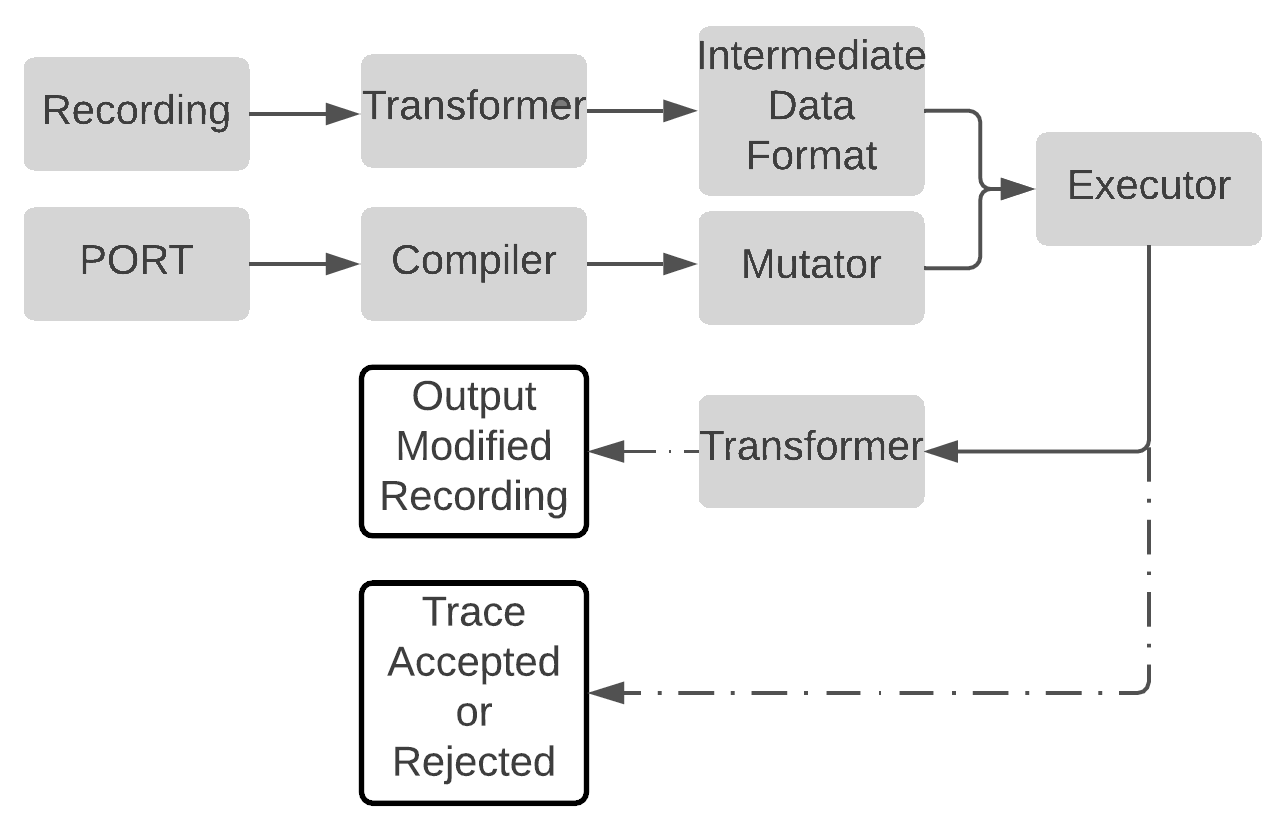
\includegraphics[scale=.08]{images/architecture}
  \caption{The CSLang compiler produces a transducer that operates over a
  generic internal data format that contains the contents of an application
  recording.}
  \label{fig:architecture}
\end{figure}

\subsection{The CSlang Compiler}

The CSlang compiler is responsible for constructing a CSlang transducer
from a CSlang program.  Once constructed, this automaton is serialized to
disk so that it may be stored and reused.
We made the decision to make CSlang a compiled language because
experience has shown that CSlang programs are typically
compiled a few times during construction
and executed many times over many different applications.
By compiling ahead of time we save the performance cost associated with other
approaches like just-in-time compilation or execution via an interpreter.


\subsection{Supporting Many Activity Representations}

In order to take the SEA technique beyond system calls we wanted to make
CSlang flexible enough that it could work with many different sorts of
activity representations.
To achieve this objective we needed to cleanly separate the details of how
an application's activity was recorded from the representation that will be
processed by a CSlang transducer.
Our solution was twofold.  First, we developed an internal data format
(IDF) that
could store the key components, such as parameter and return values,
of application activities like function
calls and system calls.  This format supports primitive string and numeric
values as well as arbitrarily nested structures in the form of records.
These decisions were based on the Linux kernel's system call implementation
which allows system call inputs and outputs in the form of primitive data
values and complex C structures.
If CSlang were going to support system calls, these capabilities would be
necessary and, further, we found that the same capabilities allowed us to
support other activity representations.

The second component is the set of modules, known as transformers, that can
convert an activity stream from its original representation into IDF and
back.  A transformer achieves the former by parsing each activity entry,
extracting the relevant fields, and assembling this information into an IDF
record.  These records are re-assembled into a stream which is input into a
CSlang transducer.  The result of processing this stream undergoes the
reverse.  The output IDF stream is converted by a transformer back into the
original activity representation.  The current version of CSlang ships with
three transformers:
\begin{itemize}
\item{strace via Posix-Omni-Parser}
\item{JSONRPC via Python's json module}
\item{XMLRPC via Python's lxml module}
\end{itemize}


\subsection{Executing a CSlang Program}

Unlike an executable program, a compiled CSlang program is a static entity
that cannot run by itself.  Instead, a component we refer to as the
``CSlang Executor'' is responsible for carrying out the ancillary work
required to analyze an application recording with a CSlang transducer.
These tasks include deserializing a stored transducer from disk, converting
the selected input stream to CSlang's internal data format using an
appropriate transformer, translating the output stream back to the original
activity representation, and reporting whether the input sequence was
accepted or rejected by the transducer. 

%\begin{itemize}
%  \item{Language describing anomalies}
%  \item{Formal model of transducer that can implement anomalies}
%  \item{Tool to compile description into said formal transducer}
%  \item{Format-agnostic intermediate data structure (IDS) over which transducer
%  operates}
%  \item{Translation layer for converting to and from concrete data into IDS}
%\end{itemize}

\subsection{Nuts and Bolts}


\section{Evaluation}
\label{SEC:evaluation}

With our prototype in hand we organized a set of
evaluations that would let us know if the PORT would be effective
in real world situations.
We designed our tests to answer the following questions:

\begin{itemize}

    % Re-implementing CS anomalies
  \item{Can PORT express the sorts of anomalies used by SEA to identify
    bugs?}

    % Extending to support RPC formats
  \item{How easy is it to extend PORT to support activity representations
    other than system calls?}

    % Dornhackl et al. defining maliciousness
  \item{What sorts of problems can be addressed by employing PORT on
  non-system-call activity representations?}

    % Performance information
  \item{Can PORT process input streams in a reasonable amount of time?}

\end{itemize}


\subsection{Expressing SEA Anomalies}
\label{sub:SEAAnomalies}
Given that this work was motivated
in large part
by the effectiveness of the SEA technique,
our first test of PORT was using it to reproduce the anomalies described
in the original paper.
We wanted to ensure that
the language we developed
would be sufficiently powerful
to describe the anomalies the
SEA research team used to
find bugs.
Specifically,
we set out to test PORT's ability to recreate
the study's Unusual Filetype mutator,
and its Cross-disk file move checkers, which were used to identify
the bulk of
the bugs that were found.
Our hope was that by using PORT we could eliminate boiler plate code,
save effort by handling common tasks automatically, and improve reliability
by providing a structured way to modify and output system call sequences.

\begin{figure}[H]
\centering
\begin{tabular}{c}
\begin{lstlisting}
event statbuf {mode: String@2};
event anystat {stat sb: statbuf@1}
        | {lstat sb: statbuf@1} | {fstat sb: statbuf@1};
anystat({sb: {mode: ->"st\_mode=S\_IFBLK"}});
\end{lstlisting}
\end{tabular}
\caption{This program identifies a stat, lstat, or fstat call and modifies
  the ST\_MODE member of its statbuf output parameter to contain the value
  "S\_IFBLK."  This indicates that the file being examined is a block device
  rather than a regular file.}
\label{lst:UnusualFiletypePORT}
\end{figure}

\subsubsection{Creating the Unusual Filetype Mutator}
\label{subsub:UnusualFiletype}
For the first phase of this work,
we used PORT to implement an ``Unusual Filetype''
mutator.
This mutator, presented in
Figure~\ref{lst:UnusualFiletypePORT},
should take an input trace
that contains a call to either {\tt stat()},
{\tt fstat()},
or {\tt lstat()}
and modify the call's result data structure such
that its {\tt ST\_MODE} member will contain a value
that indicates an unusual filetype.
Table~\ref{tbl:ST_MODEValues}.  As can be seen in
Figure~\ref{lst:UnusualFiletypePORT}, PORT's semantics mean such an
operation can be captured with only a handful of lines of code.  In the
figure
lines 1 through 4 define what {\tt stat()}, {\tt fstat()}, and {\tt
lstat()} calls look like and which parameter contains the result buffer.
Line 6 generates an accepting state that, when entered, produces an output
system call with a modified value in the return structure's {\tt st\_mode}
field.  Such output can then be used to modify the results of a running
application's system calls in order to carry out the remaining steps of the
SEA technique.

PORT's advantages are made even more obvious when the PORT Unusual
Filetype mutator is compared to a program that implements the same
functionality in a general purpose programming language like Python.
Figure~\ref{lst:UnusualFiletypePython} shows an excerpt from a 55 line
Python program taken from the SEA paper's CrashSimulator that performs the
same mutation described above.  Comparing this listing to
Figure~\ref{lst:UnusualFiletypePORT} shows several key differences:

\textit{Minimal boilerplate code:} The PORT program lacks the boilerplate
code associated with
reading an input trace, managing mutator state, and producing output.
This is possible because PORT's capabilities are narrowly defined to
only describe the states and operations of a mutator.  This means these
functions can be generically implemented within PORT's core eliminating
the need for users to do so manually.

\textit{No code required to filter out uninteresting calls:}
PORT's user does
not need to write any code to exclude system
calls outside of the desired set.  Each statement defines a new state with
incoming and outgoing transitions configured such that any system calls not
dealt with in the PORT program are ignored.

\textit{Easy to modify call contents:}  PORT's operators make it
trivial to change components of a system call
and produce output without having to regenerate the remainder of its
parameters.
This is a far cry
from the Python program which relies on manual, fragile string manipulation
to achieve the same effect.


\begin{figure}[H]
\centering
\begin{tabular}{c}
\begin{lstlisting}[language=python]
... 3 lines omitted ...
class UnusualFiletypeMutator(GenericMutator):
  def \_\_init\_\_(self, filetype='S\_IFREG', name=None, file\_descriptor=None):
  ... 6 lines omitted ...

  def mutate\_syscalls(self, syscalls):
    index = self.\_find\_index(syscalls)
    for i in range(len(syscalls[index].args)):
      if 'st\_mode' in str(syscalls[index].args[i].value):
        syscalls[index].args[i].value=re.sub(r'S\_IF(\w*)', self.filetype, syscalls[index].args[i].value)

... 13 lines omitted ...

  def identify\_lines(self, tm, que, thread\_condition):
    while True:
      ... 3 lines omitted ...
      if syscall\_trace['syscall'].name.startswith('fstat'):
        if self.file\_descriptor:
          if self.file\_descriptor != syscall\_trace.args[0].value:
            continue
        self.opportunity\_identified(syscall\_trace, self.mutator\_name, que)
      if syscall\_trace['syscall'].name.startswith('stat') or syscall\_trace['syscall'].name.startswith('lstat'):
        if self.name:
          if self.name != syscall\_trace.args[0].value:
            continue
        self.opportunity\_identified(syscall\_trace, self.mutator\_name, que)
\end{lstlisting}
\end{tabular}
\caption{This is a Python module taken from SEA's CrashSimulator that
  implements the ``Unusual Filetype'' anomaly.  This listing has been
  shortened by removing CrashSimulator specific-code so that a fair
  comparison can be drawn between it and the same mutator implemented in
  PORT.}
\label{lst:UnusualFiletypePython}
\end{figure}

\subsubsection{Creating the Cross-Disk Move Checkers}

The second phase of this work involved the recreation of a set of
``checkers'' that could examine an application as it moved a file from one
disk to another and report whether or not the operation was carried
out correctly.  These checkers took advantage of the fact that the Linux
{\tt rename()} system call does not support moving files from one disk to
another.  This means applications have to perform this complex
operation manually.  Earlier work on the SEA technique
identified XX steps required to
correctly perform such a move by examining the source code of the ``mv''
command.  With this knowledge, they
implemented a set of checkers to identify situations where one
or more of these steps were not carried out correctly.
When applied to real world applications,
these checkers were able to identify bugs
in many popular applications and libraries that offered file movement
capabilities.

Similar to the Unusual Filetype described in
Section~\ref{subsub:UnusualFiletype},
we first implemented the
set of checkers in PORT.  Figure~\ref{lst:Cross-DiskMovePORT} shows one
such checker that ensures {\tt fstat} is used after a file is opened but
before it is moved.  This pattern indicates that an application may be
storing the {\tt inode} number of the file -- a step necessary to prevent a race
condition where the file is replaced during the move process.  When
we compare this checker to the Python version in
Figure~\ref{lst:Cross-DiskMovePython} many of the qualities we discussed
above are apparent.  The PORT version is more concise and its meaning is
less obscured by boilerplate and state management code that makes up the
bulk of the Python version.

This exercise did expose one of PORT's shortcomings.
The Python checker in Figure~\ref{lst:XattrsPython},
which ensures an application
preserves all of a file's extended attributes and re-applies them the
destination file after the move.
The difficulty creting this checker
in PORT was due to two factors.
First, PORT does not support looping with a
runtime-defined number of iterations.  This is necessary to capture all
calls to {\tt getxattr()}.
Further, PORT does not support a list data structure to store the values
retrieved by such calls and ensure they have all been applied with a
corresponding call to {\tt setxattr()}.
We are evaluating these deficiencies and plan to address them in the
future.

\begin{figure}[H]
\centering
\begin{tabular}{c}
\begin{lstlisting}[language=c,showstringspaces=false]
\\ This is absolutely a fake listing that will be changed out for a real
\\ one!!  Preston -> Don't forget to do this!
#include "stdio.h"

int main() {
    printf("Hello world!\n");
    return 0;
}
\end{lstlisting}
\end{tabular}
\caption{One of the cross disk move checkers implemented in PORT}
\label{lst:Cross-DiskMovePORT}
\end{figure}


\begin{figure}[H]
\centering
\begin{tabular}{c}
\begin{lstlisting}[language=c,showstringspaces=false]
\\ This is absolutely a fake listing that will be changed out for a real
\\ one!!  Preston -> Don't forget to do this!
#include "stdio.h"

int main() {
    printf("Hello world!\n");
    return 0;
}
\end{lstlisting}
\end{tabular}
\caption{One of the cross disk move checkers implemented in Python}
\label{lst:Cross-DiskMovePython}
\end{figure}

\subsection{Extending PORT to Other Activity Representations}

While the above results are encouraging, we wanted to ensure that PORT's
usefulness was not limited to system call manipulation.
A logical next step would be to test PORT's capabilities when working
with a higher level, but similarly structured, activity representation.
After some consideration we settled on JSONRPC and XMLRPC.  These formats
were ideal because they are well defined, popular, and both have well
supported parsing libraries or modules.

To evaluate PORT's ability to work with these representations we
constructed transformer modules that could convert these formats into our
intermediate data format.
We tested our implementation by writing PORT programs that could modify
activity streams similar to the examples presented in the JSONRPC
2.0~\cite{jsonspec} and XMLRPC~\cite{xmlspec}
specifications.  One such program is shown in
listing~\ref{lst:JSONProgram}.  This program matches a pattern of ``test''
and ``update'' calls and, if the pattern is found, the final update call's
parameters are replaced with the contents of two registers.

JSONRPC support required handful of hours of effort and XMLRPC
support, whose implementation we precisely timed, was completed in three
hours and thirty-two minutes.  Based on the ease and speed with which we
ere able to complete these additions we are confident that PORT can be
quickly adapted to support new activity representations as required.

\begin{figure}[H]
\centering
\begin{tabular}{c}
\begin{lstlisting}
event update {up1: Number@0, up2: Number@1};
event test {tp1: Number@0, tp2: String@1};
update({up1: pone, up2: ptwo});
test({tp1: 45, tp2: "alpha"});
update({up1: ->999, up2: ->888});
\end{lstlisting}
\end{tabular}
\caption{This PORT program matches a pattern of JSONRPC calls to
  ``update'' and ``test.''  If the pattern is identified, the final call to
  update is modified so that its first two parameter values are replaced
  with the values stored in the outone and outtwo registers.}
\label{lst:JSONProgram}
\end{figure}


\subsection{Utilizing PORT's Flexibility}
In addition to novel formats, we wanted to see if PORT could be used to
represent proven-useful models from other work.  One candidate for this
effort is the work on describing malicious behavior done by Dornhackl et
al. in 2014~\cite{Dornhackl2014}.  This work improves upon static malicious
behavior detection using signatures by creating formal models that can
detect misbehavior in an application's dynamic activity.  This is done
using two models: one that describes malicious activity in the form of a
series of tasks and a second that maps these tasks onto the concrete
Windows API calls required to carry out these tasks.

PORT is particularly well suited to implementing the second model.  This
requires a mechanism for first grouping a set of similar API calls
into a single operation and then describing a malicious task in terms of
these aggregate operations.  PORT supports the former using variants.
For example, the work proposes grouping the API calls that may be used to
open a Windows registry key as is shown in Figure~\ref{lst:DornhacklOpen}.

\begin{figure}[H]
\centering
\begin{tabular}{c}
\begin{lstlisting}
OPEN => RegOpenKeyA NtOpenKey
  | RegOpenKeyW NtOpenKey
  | RegOpenKeyExA NtOpenKey
  | RegOpenKeyExW NtOpenKey
\end{lstlisting}
\end{tabular}
\caption{Grouping of Windows API calls for opening or creating a Windows
  registry key into an OPEN operation as per Dornhackl et al.}
\label{lst:DornhacklOpen}
\end{figure}


In the above grammar, each symbol beginning with ``Reg'' represents a user
API that opens or creates a registry key.  {\tt NtOpenKey} always follows
each of these calls because it is the underlying ``native'' call that
Windows makes to actually perform the operation.
The grouping and execution semantics for this operation can be expressed
in PORT as shown in Figure~\ref{lst:PORTOpenReg}.


\begin{figure}[H]
\begin{lstlisting}[gobble=2]
  event open {RegOpenKeyA ...} | {RegOpenKeyW ...};
    # ... further varients omitted
  event NtOpenKey {...};

  open({...});
  NtOpenKey({...});
\end{lstlisting}
  \caption{Abstract PORT program (with parameters
  omitted) that groups the Windows API calls responsible for opening or
  creating a Windows registry key into an open operation.  It also shows
  how the requirement that NtOpenKey follow any of these calls can be
  captured.}
\label{lst:PORTOpenReg}
\end{figure}

Dornhackl et al. used this strategy to describe a pattern that, if
detected, would indicate
a Windows registry key was being installed
that would cause some malicious action
the next time the machine was restarted.  We can use PORT to group the
Windows API calls into the same operations as the original work and
construct a program that could perform this detection (assuming PORT were
extended to support Windows).  Such a program appears in
Figure~\ref{lst:PORTRegDetect}.  This program groups API calls into OPEN,
SET, and CLOSE operations and searches for a pattern that
indicates
an application is
setting an autostart key.  The PORT program is further able to express
that the pattern must appear for a specific registry key using the value
stored in the ``regkey'' register.

\begin{figure}[H]
\centering
\begin{tabular}{c}
\begin{lstlisting}[gobble=2]
  event open {RegOpenKeyA ...} | {RegOpenKeyW ...} | ...;
    # further variants omitted
  event NtOpenKey {...};
  event set {RegSetValueExA ...} | {RegSetValueExW ...}
            | ...;  # further variants omitted
  event NtSetValueKey {...};
  event close {RegCloseKey ...};
  event NtClose {...};

  open({...});
  NtOpenKey({...});
  set({...});
  NtSetValueKey({...});
  close({...});
  NtClose({...});
\end{lstlisting}
\end{tabular}
  \caption{This listing shows an abstract PORT program (with parameters
  omitted) that detects situations where an application is maliciously
  installing an ``autostart'' Windows registry key.  It does so by
  implementing the pattern described by Dornhackl et al.  Unimportant
  parameters are omitted and the number of API calls in each group has been
  reduced in order to save space.}
\label{lst:PORTRegDetect}
\end{figure}


\subsection{PORT's Performance}

It doesn't matter how useful a tool may be
if it takes too long to complete its work.
Though our implementation is
only a prototype, we wanted to make sure that its performance was not
overly slow.
Our performance evaluation
is focused on the time required
to identify specific
patterns within real world system call traces.
We recorded test traces
from two popular network applications -
NCat,
and
Python's http.server.
These
were chosen because they are widely used and
offer increasing levels of complexity against which we can evaluate
PORT's effectiveness.

Our test operated as follows.  The applications were configured to service
a simple piece of content (a single string in the case of NCat) and were
recorded using {\tt strace} while handling a request from a remote client.
The strace
recordings\footnote{Recordings were pre-processed to remove system calls
related to executable loading and process creation} were then processed using the PORT program from
Figure~\ref{lst:RealWorldPerformance},  which
identified the sequence of system calls that implement
a server's request handling
loop.  Table~\ref{tbl:RealWorldPerformance}
shows the times in seconds required to perform this identification on each
web server as well as the total number of system calls in each trace.

\begin{figure}
  \begin{tabular}{|c|c|c}
                & Time in Sec. & Num. Syscalls.\\
              \hline
  http.server   & 0.104 Sec.   & 297   \\
  NCat          & 0.092 Sec.   & 43      \\
\end{tabular}
\caption{Time in seconds to process the listed number of events of each format.}
\label{tbl:RealWorldPerformance}
\end{figure}

\begin{figure}[H]
\centering
\begin{tabular}{c}
\begin{lstlisting}
event accept { accept fd: Number@ret} | { accept4 fd: Number@ret};
event anyrecv { recvfrom fd: Number@0} |
  { read fd: Number@0} |
  { recv fd: Number@0};

event anysend {sendto fd: Number@0}
  | { write fd: Number@0}
  | { send fd: Number@0};

event close {fd: Number@0};

accept({fd: !storefd});
anyrecv({fd: ?storefd});
anysend({fd: ?storefd});
close({fd: ?storefd});
\end{lstlisting}
\end{tabular}
\caption{This PORT program matches patterns where a server application
  accepts a connection, receives a request, sends a response, and closes
  the connection.  The program uses variants to handle cases where
  applications use different system calls to perform some common action
  (e.g. receiving data from a socket)}
\label{lst:RealWorldPerformance}
\end{figure}

The results in Table~\ref{tbl:RealWorldPerformance} show that, as expected,
PORT's
processing time increases in line with the total number of system calls
present in a recording.  We anticipate that much of this processing cost is
associated with setting up a Python execution environment and that a more
optimized implementation could improve performance gains in this area.
Further,
it is likely that PORT's performance is closely tied to
disk throughput,
and that advancing the mutator
as each system call is evaluated
adds little additional overhead.
A condition with varying disk
speeds could be designed to confirm this suspicion.  As a whole, our
results indicate that PORT's performance is not a limiting factor to its
usage in real-world situations.

%%% Local Variables:
%%% mode: latex
%%% TeX-master: "paper"
%%% End:

\section{Related Work}
\label{SEC:related-work}

PORT is a declarative domain-specific language designed to
assist developers in creating
applications that need to pattern match and perform
transformations on a single stream of possibly infinite events.
Potential applications
of PORT could include
processing streams of system calls, RPC invocations or
web-browser events for the purpose of intrusion detection, fault-injection, or
other program-level testing. In the following, we discuss
related work in the area of system call processing applications,
and event stream processing languages and algorithms.

\subsection{System Call Stream Processing Applications}
The
initial motivation for the development of PORT was to create a tool to help
developers express match and transformation rules for system call patterns in
CrashSimulator~\cite{DBLP:conf/issre/MooreCFW19}.

System call pattern
is an established technique
matching in intrusion detection.
Broadly speaking, there are two
different types of system call based intrusion detection systems: misuse
intrusion detection and anomaly detection. Misuse intrusion
detection systems,
search for known patterns of application-specific malicious system call
sequences known as intrusion signatures~\cite{GARCIATEODORO200918}.
In anomaly
detection that the intrusion signatures are unknown,
but any deviation
from “normally observed” system call sequences are flagged as
malicious~\cite{DBLP:conf/sp/ForrestHSL96}.
As misuse intrusion detection systems are only
effective against previously known intrusion signatures,
they are typically combined with anomaly-based systems.

Intrusion
detection systems also vary in the way in which they examine the system call
stream.
Some examine each system call in isolation,
without regard to previous
execution context,
looking for specific arguments that may imply malicious
intent.
Others look for fixed patterns or sequences of system calls executed
within a certain window of instructions.  Some of the more prominent studies in
this area are highlighted below.

Forrest et al.~\cite{DBLP:conf/sp/ForrestHSL96} describe
an anomaly detection system based on the premise that small deviations from
an application's previously exhibited system call execution pattern are likely
malicious. An application to be protected using this mechanism is first
``exercised'' on various inputs to expose the
sequence of system calls found in valid uses of the application.
Using a sliding
window of fixed size,
each witnessed pattern of contiguous system calls appearing in the system call stream is cataloged in a database. After the
training phase, the application's system call stream
is monitored and any detected
deviation from the expected system call patterns (stored in the database) are
acted upon in accordance with a predefined security policy.
Warrender et al. implemented a hidden Markov model
based implementation of this same system~\cite{DBLP:conf/sp/WarrenderFP99}.

Sekar et al.\cite{DBLP:conf/sp/SekarBDB01} extend the work
of~\cite{DBLP:conf/sp/ForrestHSL96} by proposing an algorithm and associated
optimizations to create a finite state automaton that can learn the valid system
call sequences of an application.
The automaton is not limited to recognizing the small system call sequence sizes
proposed in~\cite{DBLP:conf/sp/ForrestHSL96}.
Instead, the automaton learns the entire sequence of system calls produced by
each run of the application.
To help minimize the size of the automaton, the authors incorporate program
counter information to recognize loops.
%In addition, system calls made within standard libraries (such as libc) are excluded from the automaton as the authors felt that these system calls do not necessarily help capture the unique nature of system call behavior within the program.

The work of Ko et al.~\cite{DBLP:conf/acsac/KoFL94} describe a real-time intrusion detection system
based on simple predicate logic and regular expressions. Each system call in the
steam is converted to a standard audit-policy record format which is then
matched against program policy. For example,
the rule \lstinline+exec "/bin/(sh | csh)"+ allows a new shell to be invoked and the rule
\lstinline+~read("/etc/passed")+ prevents the password file from being read.
However, the audit-policy can only be applied to
one system call at a time, rules to recognize specific chains of system calls
are not supported.

Systrace~\cite{DBLP:conf/uss/Provos03} supports fine-grained process confinement
via system call monitoring and an associated policy language consisting of a set
of rules and triggers that execute once a rule evaluates to true.
Rules are
checked against only one system call at a time.
As Systrace intercepts each system call prior to execution, this system can also
be used for fault injection in various testing scenarios.

Similar to system calls, remote procedure calls can also be abused for malicious
intent,
so examining and acting upon a remote procedure call stream can help mitigate or prevent such attacks.
The remote procedure call protection mechanism described in~\cite{DBLP:conf/uss/GiffinJM02} uses push-down automata to model the possible valid remote call streams that can be generated in a particular application.
The model is created by static binary analysis and modification of the application to be protected.
The application's incoming remote procedure call stream is vetted against the previously created model to determine whether particular calls are valid and therefore executable.

Phoebe~\cite{DBLP:journals/corr/abs-2006-04444} is a fault-injection framework
that examines the system call stream of an application to determine which system
calls fail naturally (during normal program execution). Based on this failure
pattern,
it generates fault-injection experiments designed to test the reliability of
an application when a failure occurs. These experiments are meant to magnify the
frequency of rarely occurring system call failures and to introduce them at
points where they had not previously occurred within the application.
Only single system call matching is done - there is no facility to create
more elaborate fault-injection tests that are triggered after a specific
sequence of system calls are seen.

In~\cite{DBLP:conf/icse/ChristakisEG017}, Christakis et al. describe a
domain-specific language and runtime to allow developers to intercept and modify
Windows applications’ dynamic link library function calls (which includes system
calls). The domain-specific language provides a mechanism to identify which
function call, or, using pattern matching, set of function calls, should be
intercepted by the runtime. Once intercepted, code written in the
domain-specific language (which, in part, is a subset of the C programming
language) can be executed. This system allows one to test for and simulate
application errors in a language-agnostic manner, as the runtime operates at the
level of the application binary. The domain-specific language is only meant to
match and intercept single function calls and was not designed to trigger a code
injection only when a specific sequence of function calls are matched.

Intrusion detection via system calls is one area where we believe PORT might be useful.
The systems outlined above were built to solve one particular problem (intrusion detection via system calls) well and
therefore lack the flexibility that drove the creation of PORT.
For example, these systems were not designed to be easily retargeted
to a different type of event stream or allow transformations on the event stream.


\subsection{Event Stream Processing Languages and Algorithms}

A streaming application
is a computer program
that consumes and/or
produces
a stream of events (messages or other form of application-specific data).
A domain-specific language designed for expressing streaming applications
is referred to as a
stream processing language~\cite{DBLP:journals/sigmod/HirzelBBVSV18}.
PORT clearly
fits within the above definition.
Therefore, in this
section we look at previous work related to stream processing languages.

Pattern matching
over event streams is a paradigm
wherein a stream of continuously arriving events are examined for
possible matches against a previously defined set of rules,
which collectively form a pattern.
Languages for pattern matching over event
streams are significantly richer than languages for regular expression
matching~\cite{DBLP:conf/sigmod/AgrawalDGI08}.
Stream processing languages typically provide automatic
support for naming, type checking, filtering, aggregating, classifying and
annotation of incoming events, and provide many benefits over traditional
stream-based text processing languages such as sed~\cite{Mcmahon1979sed} and
awk~\cite{DBLP:journals/spe/AhoKW79}.

Although PORT is a stream processing language, it does not
require all of the features typically
provided by many stream processing systems, such as
combining multiple stream sources,
out of order data retrieval,
methods for handling data loss,
time window based event aggregation,
or database integrations~\cite{DBLP:journals/csur/DayarathnaP18}.
Rather PORT seems to fit within the special case of
stream processing known as complex event processing (CEP),
in which data items in input streams are referred to as raw events and data items in output streams
as composite (or derived) events. A CEP system uses patterns to inspect
sequences of raw events and then generates a composite event for each
match~\cite{DBLP:journals/ibmrd/HirzelAGJKKMNSSW13}.

Queries and transforms written for CEP systems are
frequently compiled to a low-level general purpose language (C, C++, etc.) to allow for fast
processing of the stream. During the compilation process, automata are typically
built to recognize the patterns specified by the queries. For instance, Agrawal et
al.~\cite{DBLP:conf/sigmod/AgrawalDGI08} describe how patterns written in the SASE+ stream
processing language are converted to non-deterministic finite automata, which are then
optimized.

MatchRegex~\cite{DBLP:conf/debs/Hirzel12} is a CEP engine for IBM’s Stream Processing
Language. Predicates defined on the individual events appearing in the event
stream can be utilized in the regular expression-based pattern matching
engine. MatchRegex supports regular expression operators, such as “Kleene star”
and “Kleene plus” over patterns consisting of predicates (boolean expressions).
Standard regular expression semantics apply over these predicate-based patterns.

The CEP systems described in this subsection are capable
of recognizing the same stream patterns that PORT can.
However, these CEP systems do not incorporate the
stream transformation primitives required for the applications
envisioned for PORT. Although CEP systems do allow for the
generation of composite events from raw events these composite events
are meant to be utilized solely for recognition of additional patterns.
It is the combination and interplay of pattern matching and transformation
primitives that distinguishes PORT from CEP systems.


\subsection{Anomaly Detection using Deterministic/Finite State Automata}
New citations go here

%%% Local Variables:
%%% mode: latex
%%% TeX-master: "paper"
%%% End:

\section{Conclusion}
\label{sec:Conclusion}
%[Be sure to end strong!  Tell the reader why your work is important.
%Explain the few key takeaways.  Benefits, eval results, usage, what is new.]
%
%[If code / data is available, reiterate]
%
%[optionally, explain future work]

A great deal of value can be gained from the analysis of an application's
activity.
Unfortunately,
the volume of activity an application produces makes it difficult
to separate out
unimportant sequences.
In this work we demonstrate our effort to improve this sitaution through the use
of our new domain specific language - CSlang.
CSlang offers a way to write concise, but powerful,
descriptions of significant application activity sequences
that can be compiled into programs that both recognize the described sequence
within an application activity stream and modify its contents in order to
facilitate more active testing.

We have also shown how easily CSlang can be extended to support other activity
representations and several scenarios where

%As we have discussed, it is common for an application to fail upon deployment
%because of unexpected interactions with its environment. Although finding and
%eliminating faults in an application is a key concern for software developers,
%it is impractical to test it in every environment it will face. To address this
%problem, we developed Simulating Environmental Anomalies (SEA). SEA is
%beneficial for developers because it allows the effort spent debugging failures
%in a given envi- ronment to be preserved and reused programmatically to test
%whether future applications will also fail. As this process is repeated, a
%corpus of bug-causing aspects, known as “anoma- lies,” along with mutators and
%checkers that characterize these anomalies, can be accumulated. In doing so,
%developers have an ever-increasing capability to test applications in situations
%that proved problematic in the past.
%
%We built a concrete implementation of SEA called Crash- Simulator that
%implements the technique by simulating en- vironmental anomalies extracted from
%the system calls an application makes. Operating on system calls gives the tool
%a “universal” way to encode and inject anomalies. Consequently, a set of
%mutations can be collected from existing applications for use in testing others.
%Our evaluation of CrashSimulator has shown that this technique is effective at
%finding bugs in well tested software. In total, 65 new bugs were identified in
%popular applications. These bugs, if triggered in the wild, could lead to
%effects ranging from simple program hangs to security vulnerabilities and data
%loss.
%
%Given that the technique has proven effective, future work to expand its use is
%warranted. This work includes developing a public repository of anomalies that
%can be applied to new or existing applications. We are also exploring
%opportunities to further automate the discovery process and improve the way
%anomalies are specified using a domain specific language. As this research
%evolves, we will focus on analyzing how an application attempts to recover from
%the anomalies. This would allow us to determine whether an application is
%correctly recovering from an error, or carrying out some incorrect response.


\vspace{-.5cm}
\bibliographystyle{apalike}
{\small
\bibliography{bibdata}}


\end{document}
